\documentclass[a4paper]{../TPInsa}

\title{Dossier organisationnel}

\begin{document}
	\pageTitre
	\tableMatieres

		L'objectif de la société PICASO est de diversifier sa gamme de produits de façon à mieux répondre à la demande de ses clients. Nous devons aussi guider la mise en place d'un processus de gestion de production de type MRP2.	
	
	\section{Situation actuelle}
	
	\subsection{Description de l'entreprise}
	
	La société PICASO est une entreprise industrielle spécialisée dans le mobilier de salon pour les particuliers et les entreprises. La maison mère est installée à Lons-Le-Saunier. Les produits sont principalement vendus en grandes surfaces généralistes, en magasins d'ameublement et auprès des fournisseurs de mobilier de bureau. Ses savoir-faire métiers sont la découpe, le travail et l'assemblage du bois.
	
	Sur le site d'Ayze en Haute-Savoie, la société Picaso a décidé de se concentrer sur les bibliothèques basses en pin. Ce produit est très simple, intemporel et bon marché. La gamme des bibliothèques basses est composée des modèles ARM100 et ARM200, bibliothèques de respectivement 100cm et 200cm.  
	
	\fixedWidthFigure{bibliotheque_basse.jpg}{ARM100}{0.6\textwidth}
	
	L'entreprise a également tissé des relations privilégiées avec des fournisseurs en qui l'on peu avoir une confiance aveugle. 
	
	\subsection{Description du personnel}
	L'entreprise fonctionne en 1/8 : 5 jours par semaine, 8 heures par jours. Une seule équipe de production est présente 8 heures par jour sur le site d'Ayze. Cela équivaut a un total de 40 heures par personne à la semaine. 
	
	Le personnel est composé d'une dizaine d'employés : trois personnes travaillant sur la fabrication et 6 autres sur l'assemblage. 
	\subsection{Description du patrimoine matériel}
	L'usine d'Ayze est composé de plusieurs machines permettant la fabrication et l'assemblage des bibliothèques basses ARM100 et ARM200. 
	La parc de machines est le suivant :
	\begin{itemize}
	\item 3 machines de découpes : DEC1, DEC2, DEC3
	\item 3 machines de traitement du bois : MB1, MB2, MB3
	\item 1 machine d'assemblage de sous ensemble : LASE
	\item 2 machines d'assemblage final : LAF1, LAF2
	\end{itemize}
	
	Le mode de fonctionnement est actuellement du 1/8 mais il n'y aucune restriction à un fonctionnement en 2/8 (c'est à dire 16h de travail par jour).
	\section{Situation future}
	
	\subsection{Les nouvelles familles de produit}
	Nous avons choisi de créer trois nouvelles familles de produit : blocs standards, blocs thermiques/électriques, pieds. Ces trois familles correspondent aux composant principaux de la table et vont nous permettre de décrire la nouvelle charge de la production. 
	Nous présentons en dessous les nomenclatures de ces familles de produit, elles impliques l'utilisation de nouveaux postes que nous détaillerons plus loin. 
	
	\begin{figure}[H]
	\centering
	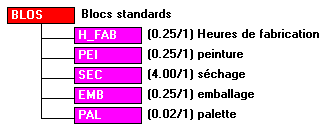
\includegraphics[scale=0.8]{captures/standard.PNG}
	\caption{Nomenclature d'un bloc standard}
	\end{figure}
	
	\begin{figure}[H]
	\centering
	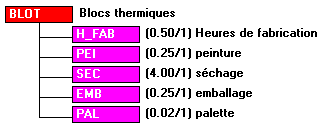
\includegraphics[scale=0.8]{captures/thermique.PNG}
	\caption{Nomenclature d'un bloc thermique}
	\end{figure}

	\begin{figure}[H]
	\centering
	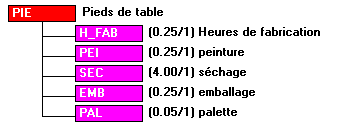
\includegraphics[scale=0.8]{captures/pied.PNG}
	\caption{Nomenclature d'un pied}
	\end{figure}
	
	\subsection{PLan commercial et plan industriel}
	
	Nous rappelons ici le plan commercial et présentons le plan industriel proposé qui permettra de répondre à la demande en lissant la production sur l'année. Nous prévoyons une progression des ventes rapide avec stabilisation à 6 mois. Les stocks seront ainsi assez hauts le premier semestre avec ensuite une diminution. L'usine est peu ouverte mois d’août, ainsi les stocks seront fortement mis à contribution durant cette période.
	
	\begin{figure}[H]
	\centering
	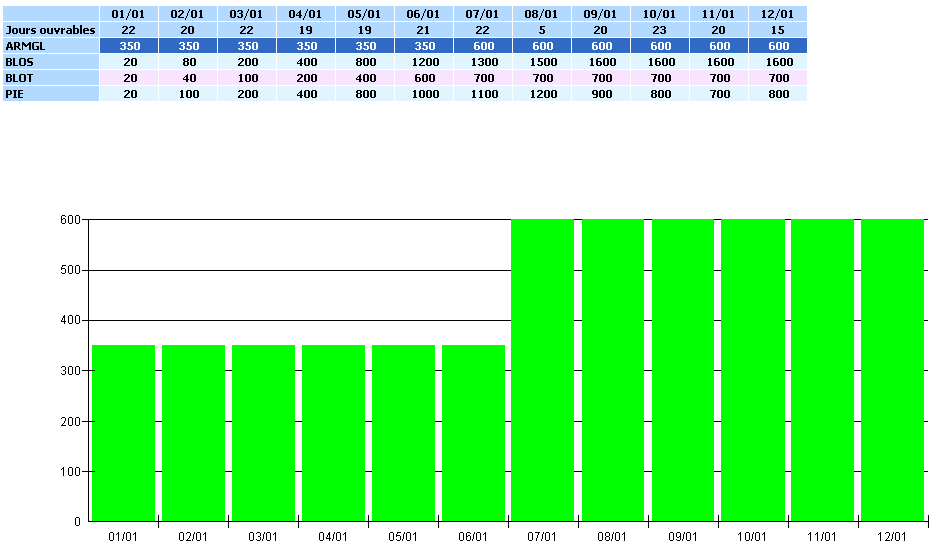
\includegraphics[scale=0.6]{captures/plan_commercial.PNG}
	\caption{Plan commercial}
	\end{figure}
	
	\begin{figure}[H]
	\centering
	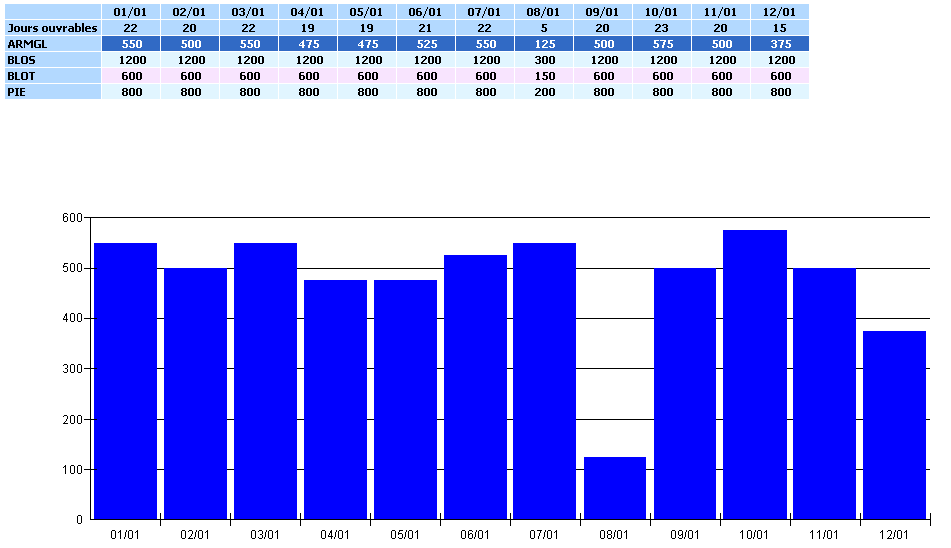
\includegraphics[scale=0.6]{captures/plan_industriel.PNG}
	\caption{Plan industriel}
	\end{figure}
	
	\subsection{Charges des postes assemblage et fabrication}
	Voici les charges prévisionnelles des postes déjà existant. L'assemblage conservera son niveau de charge actuel. La capacité de fabrication devra par contre être doublée (en hommes et machines). 
	
	\begin{figure}[H]
	\centering
	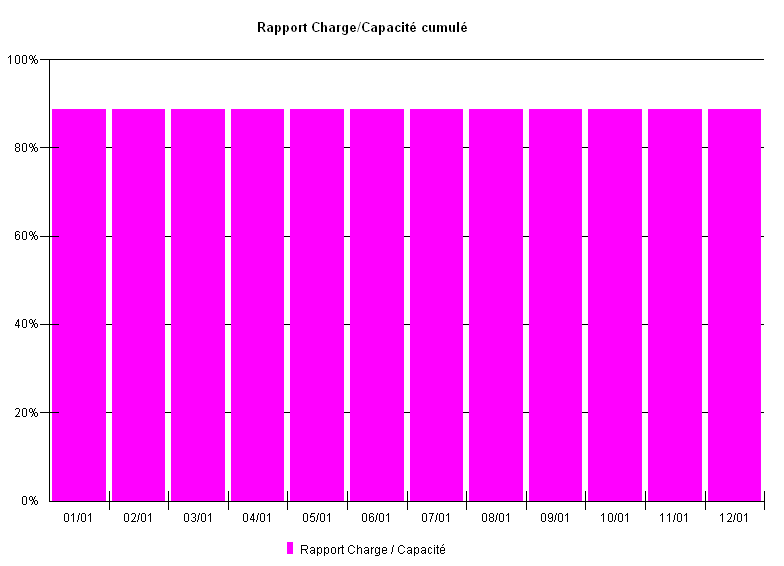
\includegraphics[scale=0.6]{captures/charge_ass.PNG}
	\caption{Charge du poste d'assemblage}
	\end{figure}
	
	\begin{figure}[H]
	\centering
	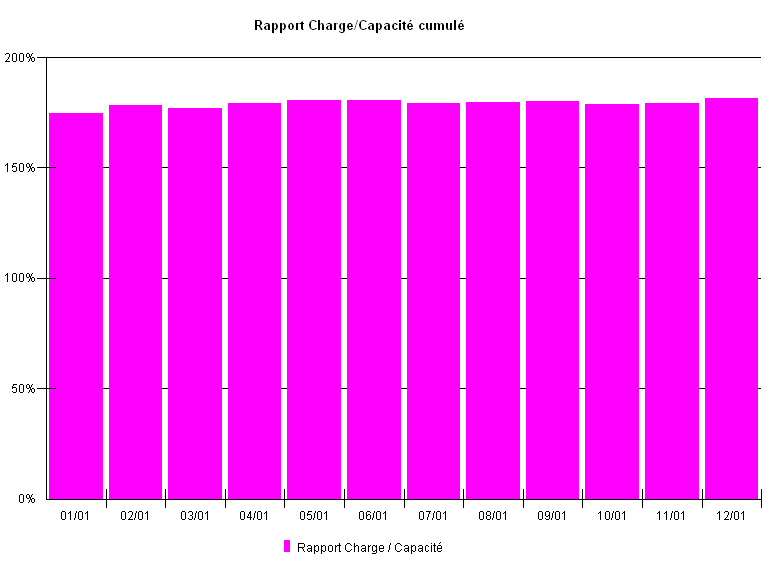
\includegraphics[scale=0.6]{captures/charge_fab.PNG}
	\caption{Charge du poste de fabrication}
	\end{figure}
	
	\subsection{Charges des nouveaux postes}
	La création de quatre nouveaux postes peut paraître importante mais il s'agit de postes génériques pouvant servir à la fabrication de multiples produits et seront donc très utile au développement à long terme de l'entreprise. 
	
	Le poste de peinture est essentiel à la mise en place de la stratégie de différenciation retardée. Quatre postes seront nécessaires ainsi qu'autant de peintres d'après le profil de charge. De plus comme décrit dans le dossier méthode, des installations spécifiques pourront être nécessaires comme des hottes pour se protéger des vapeurs de peinture, lasure etc...
	\begin{figure}[H]
	\centering
	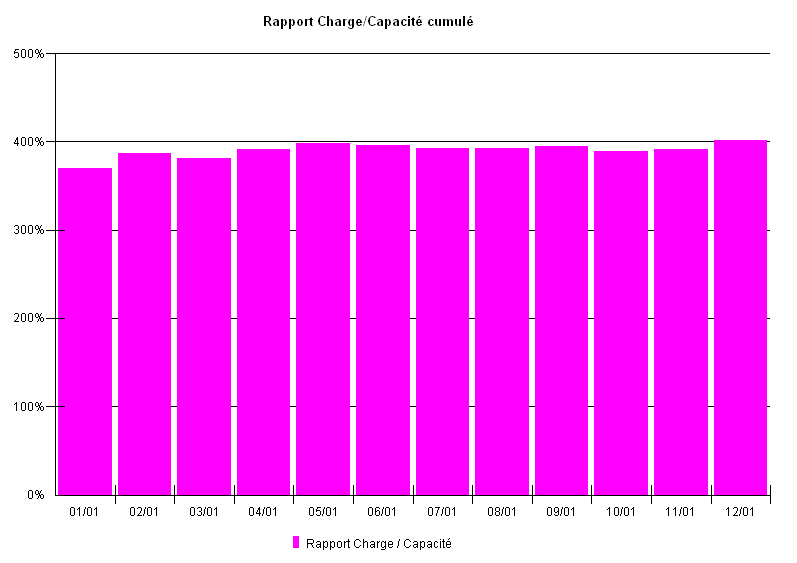
\includegraphics[scale=0.6]{captures/charge_pein.PNG}
	\caption{Charge du poste de peinture}
	\end{figure}
	
	Le poste de séchage est très chargé mais peu de place est nécessaire pour faire sécher un composant. De fait ce poste peut être aisément parallélisé en utilisant une pièce de taille importante. Un seul employé devrait être nécessaire à la bonne marche de ce poste.
	\begin{figure}[H]
	\centering
	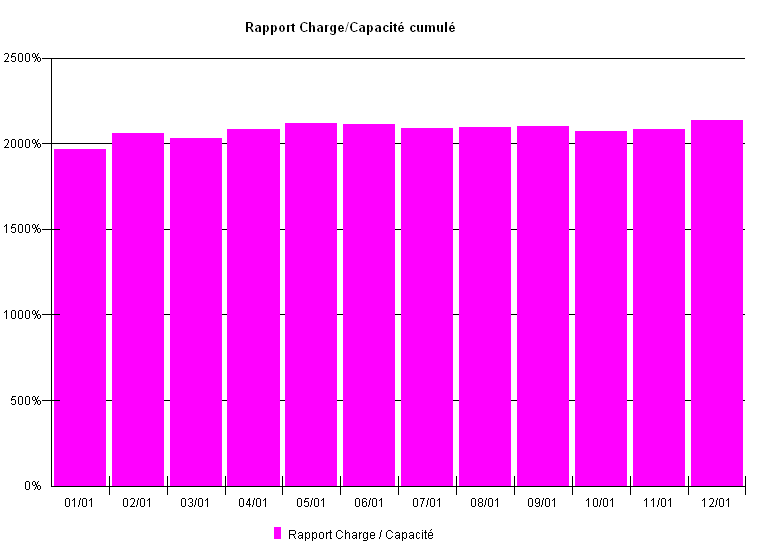
\includegraphics[scale=0.6]{captures/sechage.PNG}
	\caption{Charge du poste de séchage}
	\end{figure}
	
	Le poste d'emballage suivra la même organisation que le poste de peinture. 
	\begin{figure}[H]
	\centering
	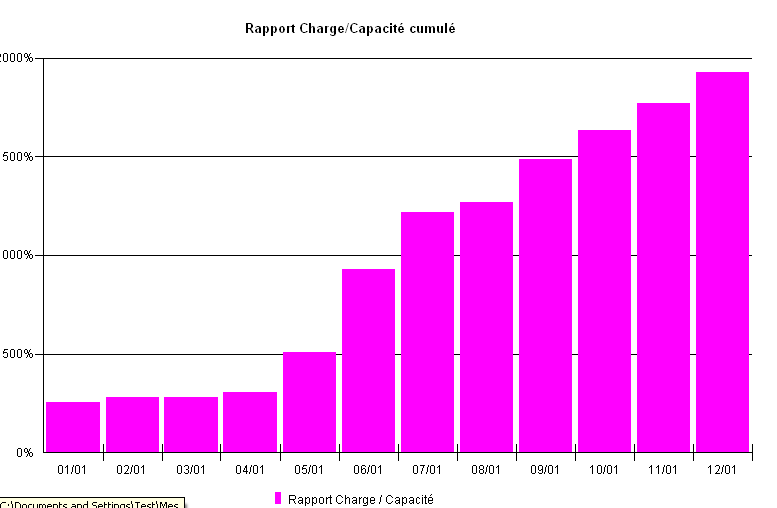
\includegraphics[scale=0.6]{captures/charge_emb.PNG}
	\caption{Charge du poste de emballage}
	\end{figure}
	
	Enfin le dernier poste, la mise sur palette, est peu chargé, on pourrait donc imaginé qu'il soit géré par une personne à temps partiel ou par quelqu'un qui travaille également sur le poste d'assemblage qui n'est pas chargé à 100\% lui non plus.
	\begin{figure}[H]
	\centering
	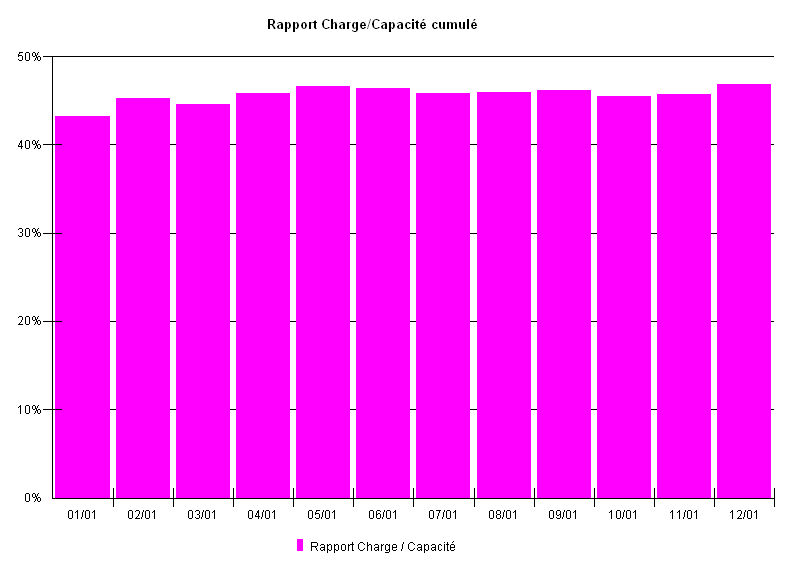
\includegraphics[scale=0.6]{captures/charge_pal.PNG}
	\caption{Charge du poste de mise sur palette}
	\end{figure}
	\subsection{Bilan des moyens humains et de production à mettre en œuvre}

	Il faut doubler les moyens de production du poste de fabrication soit ajouter 3 personnes et les machines nécessaire. 
	L'usine devra se doter de 4 postes de peintures et d'emballage, d'une pièce dédiée au séchage, d'un poste de mise sur palette ainsi que de portes palettes et de hottes (cf dossier méthodes). 
	Enfin elle devra embaucher en plus des trois personnes dédiée à la fabrication : 4 peintres, 4 emballeurs, 1 employé contrôlant le séchage et 1 autre s'occupant de la mise sur palette (à temps partiel ou travaillant aussi sur un autre poste) soit 13 nouvelles personnes en tout. 
	
	Si PICASO souhaite acheter moins de nouvelles machines, l'entreprise pourrait par exemple ouvrir plus longtemps au cours de la journée (10 ou 12 heures au lieu des 8 actuelles) pour utiliser davantage les moyens existants. 

	\section{Conclusion}

L'arrivée du nouveau produit devrait plus que doubler l'activité de l'entreprise et participer grandement à son développement. Les investissements sont importants mais nous prédisons une augmentation rapide des ventes et donc un retour sur investissement tout aussi rapide. De plus les nouveaux moyens mis en œuvre sont génériques et pourront servir dans le futur au développement de nouveaux produits. 




















	\end{document}
